%==============================================================================
%  Drone-Guided Autonomous Navigation: A Cooperative UAV--AMR System
%  for GPS-Denied Environments
%
%  Graduation Project --- Tecnológico de Monterrey
%  In partnership with OMRON Automation and Nuclea Solutions
%
%  Document class: IEEEtran (conference)
%  NOTE: Prose drawn from the per-subsystem DOCS.md sources. Figures and
%        experimental numbers are marked with \FIG{} / \TODO{} for incremental
%        insertion.
%==============================================================================
\documentclass[conference]{IEEEtran}

%------------------------------------------------------------------------------
%  Packages
%------------------------------------------------------------------------------
\usepackage{cite}
\usepackage{amsmath,amssymb,amsfonts}
\usepackage{algorithmic}
\usepackage{algorithm}
\usepackage{graphicx}
\usepackage{textcomp}
\usepackage{xcolor}
\usepackage{booktabs}
\usepackage{multirow}
\usepackage{array}
\usepackage{siunitx}
\usepackage{bm}
\usepackage{url}
\usepackage[hidelinks]{hyperref}

\usepackage{pifont}
\usepackage{tikz}
\usetikzlibrary{arrows.meta,positioning,shapes.geometric}

\newcommand{\checked}{\textcolor{green!60!black}{\ding{51}}}

\graphicspath{{figures/}}

% IEEEtran-recommended fix for \BibTeX / \LaTeX spacing
\def\BibTeX{{\rm B\kern-.05em{\sc i\kern-.025em b}\kern-.08em
    T\kern-.1667em\lower.7ex\hbox{E}\kern-.125emX}}

%------------------------------------------------------------------------------
%  Convenience macros
%------------------------------------------------------------------------------
\newcommand{\TODO}[1]{\textcolor{red}{\textbf{[TODO: #1]}}}
\newcommand{\FIG}[1]{\textcolor{blue}{\textbf{[FIGURE: #1]}}}
\newcommand{\subsys}[1]{\texttt{#1}}      % monospace package/node names
\newcommand{\Rmat}{\mathbf{R}}
\newcommand{\Tmat}{\mathbf{T}}
\newcommand{\state}{\mathbf{X}}

\begin{document}

%==============================================================================
%  TITLE
%==============================================================================
\title{Drone-Guided Autonomous Navigation: A Cooperative UAV--AMR System for
       GPS-Denied Environments}

\author{
    \IEEEauthorblockN{David Ortiz, Alfredo Romo, Noé Rosales, Sebastián Pulido, Jorge González}
    \IEEEauthorblockA{
        \textit{School of Engineering and Sciences} \\
        \textit{Tecnológico de Monterrey} \\
        Guadalajara, Mexico \\
        \TODO{emails / matrículas}
    }
}

\maketitle

%==============================================================================
%  ABSTRACT
%==============================================================================
\begin{abstract}
Many autonomous ground robots must operate where satellite positioning is
unavailable or unreliable: indoor warehouses and underground facilities receive
no signal, while container yards, dense urban canyons, and forest or disaster
sites suffer multipath, occlusion, and blockage that degrade GPS at ground level.
We present a cooperative
unmanned-aerial-vehicle (UAV) and autonomous-mobile-robot (AMR) system that
solves goal-directed navigation in such a GPS-denied setting. The two agents are
complementary: the UAV has access to absolute positioning at altitude (provided
in our testbed by a motion-capture system acting as a GPS surrogate) but cannot
transport cargo, while the AMR carries no absolute-positioning instrumentation by
design and therefore cannot independently determine the global location of its
goal. Our pipeline has the UAV survey an unmapped $4\times4$~m arena from above,
build a metric occupancy map through a similarity-transform image-stitching
pipeline, and localize ArUco goal markers in the world frame; this aerial prior
is then handed to the AMR, which fuses it with live LiDAR sensing to plan and
execute a collision-free path. Core technical contributions include a
from-scratch extended Kalman filter with an adaptive visual-odometry outlier
gate, a priority-weighted map-fusion rule, an independent automatic-emergency
-braking layer, and an application-layer cryptographic middleware securing all
inter-robot traffic. The system is implemented entirely in ROS~2 across three
networked compute platforms. \TODO{Headline quantitative results.}
\end{abstract}

\begin{IEEEkeywords}
GPS-denied navigation, cooperative robotics, UAV--AMR, ROS~2, extended Kalman
filter, image stitching, occupancy mapping, ArUco localization, autonomous
emergency braking, robot cybersecurity.
\end{IEEEkeywords}

%==============================================================================
%  I. INTRODUCTION
%==============================================================================
\section{Introduction}
\label{sec:intro}

\subsection{Motivation and Problem Context \checked}
Modern logistics increasingly relies on autonomous ground vehicles for material
transport. In structured indoor warehouses this is well understood, but a large
class of industrially relevant environments---maritime ports, container yards,
and partially enclosed industrial sites---combine the openness of outdoor
operation with the GPS degradation of dense infrastructure. At ground level,
satellite positioning in these settings suffers from multipath reflections off
metal containers and cranes, partial sky occlusion, and signal blockage, making
it unreliable as the sole basis for navigation. A robot operating there cannot
assume it knows where it is, nor where its destination lies, in any global frame.

This project targets exactly that regime: autonomous navigation toward a goal
whose global position is not known a~priori to the ground vehicle, in an
environment for which no map exists in advance.

\subsection{Problem Statement \checked}
We consider a $4\times4$~m arena populated with static obstacles and several
ArUco fiducial markers that denote goal/zone locations and visual landmarks. An AMR must navigate from
a start pose to a marked goal without colliding with obstacles. Two constraints
define the difficulty. First, no map of the arena is available before the
mission---it must be constructed at runtime. Second, the AMR carries \emph{no}
absolute-positioning instrumentation: it has wheel encoders, an inertial
measurement unit (IMU), a 2D LiDAR, and a camera, but nothing that fixes its pose
in a global frame. This is a deliberate modelling choice that mirrors the
GPS-denied ground robot of the motivating scenario. Consequently the AMR cannot,
on its own, determine the global position of a visual landmark marker it has not yet seen.

\subsection{Proposed Approach}
We resolve the deadlock through cooperation with a second agent that \emph{does}
have absolute positioning, but at altitude. A UAV equipped with a downward camera
and tracked by a motion-capture system (acting as a surrogate for the absolute
positioning a real outdoor drone would obtain from GNSS) surveys the arena from
above. From its georeferenced aerial video it (i) builds a metric occupancy grid
of the arena and (ii) localizes the ArUco goal markers in the world frame. This
aerial prior---map plus goal pose---is handed to the AMR, which fuses it with its
own live LiDAR occupancy map, plans a path with A$^\star$, and tracks that path
with a feedback-linearizing controller. Throughout, the AMR maintains a local
pose estimate from a custom extended Kalman filter (EKF) that fuses wheel, IMU,
and visual-odometry velocity, re-anchored when goal markers are observed.

\subsection{Contributions}
The system integrates a number of subsystems, each documented in depth in this
report:
\begin{itemize}
  \item A UAV position controller and scan-trajectory generator that tracks a
        boustrophedon survey pattern under motion-capture feedback, with a
        sliding-window fault detector robust to intermittent tracking dropouts
        (Sec.~\ref{sec:uav-control}).
  \item An aerial image-stitching pipeline that builds a metric occupancy map
        using a similarity-transform formulation specifically chosen to remain
        stable over the arena's repetitive grid texture, with an embedded
        deep-learning feature front-end and a learned map-quality classifier
        (Sec.~\ref{sec:stitching}).
  \item A marker-localization subsystem combining planar PnP through a $45^\circ$
        mirror rig with robust geometric-median aggregation and a calibrated
        bias model (Sec.~\ref{sec:aruco}).
  \item A from-scratch EKF with a two-stage adaptive gate that rejects the
        impulsive velocity bursts produced by visual-SLAM loop closures
        (Sec.~\ref{sec:ekf}).
  \item A priority-weighted map-fusion rule that merges the aerial prior with the
        AMR's live map without any registration step (Sec.~\ref{sec:fusion}).
  \item An independent, high-rate automatic-emergency-braking layer
        (Sec.~\ref{sec:aeb}) and an application-layer security middleware
        protecting all ROS~2 traffic (Sec.~\ref{sec:security}).
\end{itemize}

\subsection{Document Organization}
Section~\ref{sec:background} provides theoretical background.
Section~\ref{sec:requirements} states system requirements, and
Section~\ref{sec:architecture} presents the hardware and software architecture.
Section~\ref{sec:pipeline} describes the cooperative mission pipeline that frames
the subsystem deep dives in Sections~\ref{sec:uav-control}--\ref{sec:security}.
Section~\ref{sec:results} reports experimental results, and
Section~\ref{sec:conclusion} concludes.

%==============================================================================
%  II. THEORETICAL BACKGROUND
%==============================================================================
\section{Theoretical Background}
\label{sec:background}
This section collects the theory the subsystems rely on. Each primer is kept
brief; full derivations and the design choices specific to our implementation
appear in the corresponding deep-dive section.

\subsection{Differential-Drive Kinematics and Feedback Linearization}
A differential-drive (unicycle) robot has configuration $(x,y,\theta)$ evolving
as $\dot{x}=v\cos\theta$, $\dot{y}=v\sin\theta$, $\dot{\theta}=\omega$, where
$v,\omega$ are body-frame forward and angular velocity. The robot is
non-holonomic: it cannot translate instantaneously along its lateral axis. This
makes direct proportional control of the geometric centre ill-posed, because the
mapping from $(v,\omega)$ to centre velocity is singular. Feedback linearization
sidesteps this by controlling a \emph{virtual point} offset a fixed distance
$R$ ahead of the centre; the map from $(v,\omega)$ to that point's velocity is
invertible for all $\theta$, yielding linear, decoupled error dynamics
(Sec.~\ref{sec:drive}).

\subsection{The Extended Kalman Filter}
The EKF estimates the state of a nonlinear system by alternating a
\emph{prediction} step, which propagates the state mean through the nonlinear
process model $f$ and the covariance through its Jacobian $F=\partial f/\partial
\state$, with \emph{update} steps that correct the prediction using measurements
through an observation model---linear in our case, so each update reduces to the
ordinary Kalman correction. Each update computes a Kalman
gain trading off process and measurement uncertainty. Numerically robust
implementations use the \emph{Joseph form} of the covariance update, which
preserves symmetry and positive semi-definiteness regardless of gain magnitude
(Sec.~\ref{sec:ekf}).

\subsection{Bayesian Occupancy Grids}
An occupancy grid discretizes the world into cells, each holding the probability
that it is occupied. Maintaining this in \emph{log-odds} form,
$l=\log\frac{p}{1-p}$, turns Bayesian measurement integration into simple
addition: each sensor reading adds an occupied or free increment to the cells it
observes, with the cells along a range beam updated by ray casting (Bresenham).
Asymmetric increments encode that a single occupied return is more informative
than a single free return (Sec.~\ref{sec:mapping}).

\subsection{Feature-Based Image Stitching}
Stitching aligns overlapping images by detecting keypoints (e.g.\ SIFT),
matching their descriptors, and estimating a geometric transform between frames.
Spurious matches are filtered by Lowe's ratio test and by RANSAC, which fits the
transform to the largest consistent inlier set. The transform family matters: a
full projective homography has 8 degrees of freedom, whereas a \emph{similarity}
transform (translation, rotation, uniform scale) has only 4. For a nadir camera
over a planar scene the true motion is a similarity, and constraining the
estimate to that family prevents the extra projective degrees of freedom from
fitting noise---critical over repetitive texture (Sec.~\ref{sec:stitching}).

\subsection{Marker-Based Pose Estimation}
ArUco markers are square fiducials whose four corners, detected in the image,
provide 2D--3D correspondences for a Perspective-$n$-Point (PnP) pose solve. For
a planar target the problem reduces to a homography from which the pose is
recovered in closed form; the Infinitesimal Plane-based Pose Estimation
(IPPE\_SQUARE) method returns the two candidate poses of the planar ambiguity,
disambiguated by reprojection error (Sec.~\ref{sec:aruco}).

\subsection{Graph Search and Trajectory Generation}
A$^\star$ searches a grid graph for a minimum-cost path using an admissible
heuristic; on an 8-connected grid the octile distance is the tight admissible
heuristic. The resulting waypoint sequence is converted to a smooth, time
-parameterized trajectory by fitting an arc-length-parameterized cubic spline
and applying a trapezoidal speed profile, yielding continuous reference position
and velocity for the tracking controller (Sec.~\ref{sec:planner}).

\subsection{Applied Cryptography Primitives}
Message authentication and confidentiality rest on three primitives. A
public-key infrastructure (PKI) binds identities to public keys through
certificates signed by a trusted certificate authority (CA). RSA-PSS produces
asymmetric signatures giving integrity and sender authenticity. AES-256-GCM is a
symmetric authenticated cipher giving confidentiality. Combining them---sign
then encrypt at the sender, verify before decrypt at the receiver---yields a
channel that is both authenticated and confidential (Sec.~\ref{sec:security}).

%==============================================================================
%  III. SYSTEM REQUIREMENTS
%==============================================================================
\section{System Requirements}
\label{sec:requirements}

\subsection{Functional Requirements}
\begin{table}[t]
\caption{Functional Requirements}
\label{tab:fr}
\centering
\begin{tabular}{@{}p{0.07\columnwidth}p{0.78\columnwidth}@{}}
\toprule
\textbf{ID} & \textbf{Requirement} \\
\midrule
FR-1 & The AMR shall navigate from start to a marked goal in a GPS-denied arena without human intervention. \\
FR-2 & The UAV shall autonomously survey the arena and build an occupancy map prior to AMR navigation. \\
FR-3 & The system shall localize ArUco goal markers in the world frame with accuracy sufficient for planning. \\
FR-4 & The AMR shall detect and avoid static obstacles in real time. \\
FR-5 & The mission shall execute without a pre-built map; the map is built at runtime. \\
FR-6 & The system shall tolerate communication latency and degrade safely on loss. \\
FR-7 & Mission-critical ROS~2 topics shall be authenticated, and optionally encrypted. \\
FR-8 & The UAV shall fly an autonomous coverage (boustrophedon) survey trajectory under closed-loop position control. \\
FR-9 & The system shall localize the AMR in the world frame from a drone-observed top fiducial, to align the AMR \texttt{odom} frame with \texttt{world}. \\
FR-10 & The AMR shall fuse its proprioceptive and onboard sensors (wheel, IMU, visual odometry) into a single continuous pose estimate. \\
FR-11 & The system shall assess aerial-map quality automatically and fall back to autonomous frontier exploration when the map is rejected. \\
FR-12 & The system shall halt the AMR on imminent collision independently of, and faster than, the planning loop. \\
FR-13 & The AMR shall accommodate slowly moving obstacles through continuous occupancy-map updates (degraded, non-predictive handling). \\
\bottomrule
\end{tabular}
\end{table}

\subsection{Non-Functional Requirements}
\begin{table}[t]
\caption{Non-Functional Requirements}
\label{tab:nfr}
\centering
\begin{tabular}{@{}p{0.07\columnwidth}p{0.78\columnwidth}@{}}
\toprule
\textbf{ID} & \textbf{Requirement} \\
\midrule
NFR-1 & The state estimator shall be implemented from scratch (no off-the-shelf localization package). \\
NFR-2 & The LiDAR occupancy map shall update at $\geq 0.5$~Hz. \\
NFR-3 & The planner shall replan within \SI{500}{\milli\second} of a new map. \\
NFR-4 & The AEB layer shall react to obstacles within ${\sim}\SI{333}{\milli\second}$ at the deployed LiDAR rate. \\
NFR-5 & The stitching pipeline shall fit within the Jetson Orin Nano's \SI{8}{\giga\byte} memory. \\
NFR-6 & The system shall run on ROS~2 Humble. \\
NFR-7 & The EKF and tracking-control loops shall run at \SI{100}{\hertz}. \\
NFR-8 & The compute shall be decentralized across at least two independent on-board processors (RDK~X3, Jetson Orin Nano). \\
NFR-9 & Inter-machine map and goal topics shall use latched (\texttt{TRANSIENT\_LOCAL}) QoS so late-joining nodes receive them. \\
NFR-10 & The security layer shall be globally disengageable through a single kill switch without code changes. \\
NFR-11 & Per-message cryptographic overhead shall remain within the real-time messaging budget. \\
\bottomrule
\end{tabular}
\end{table}

\subsection{Mechanical and Electronic Requirements}
\begin{table}[t]
\caption{Mechanical and Electronic Requirements}
\label{tab:er}
\centering
\begin{tabular}{@{}p{0.07\columnwidth}p{0.78\columnwidth}@{}}
\toprule
\textbf{ID} & \textbf{Requirement} \\
\midrule
ER-1 & The AMR LiDAR scan plane shall sit at \SI{13}{\centi\meter}---above floor discontinuities, below obstacle height. \\
ER-2 & The UAV shall view the arena at nadir via a $45^\circ$ mirror redirecting its forward camera. \\
ER-3 & The static transform $\texttt{base\_footprint}\to\texttt{lidar}$ shall be $x=\SI{0.07}{\meter}$, $z=\SI{0.13}{\meter}$. \\
ER-4 & The camera-to-drone transform shall be calibrated once per deployment (roll $=\pi$, yaw $=\SI{0.0456}{\radian}$). \\
\bottomrule
\end{tabular}
\end{table}

%==============================================================================
%  IV. SYSTEM ARCHITECTURE
%==============================================================================
\section{System Architecture}
\label{sec:architecture}

\subsection{Hardware Platform}
The ground robot is built on a Yahboom RDK~X3 differential-capable base
(quad-core ARM Cortex-A53) carrying an NVIDIA Jetson Orin Nano (\SI{8}{\giga\byte}
RAM, GPU) as a compute co-processor. Its sensors are an OraDAR MS200 2D LiDAR
($360^\circ$, \SI{15}{\hertz}, \SIrange{0.05}{20}{\meter}), an integrated IMU and
wheel encoders read over the SunriseRobot SDK, and a forward facing Intel Realsense D435i camera used for
fiducial detection and Visual Simultaneous Localization and Mapping (VSLAM). The aerial agent is a DJI Tello quadrotor with downward and
forward cameras; a $45^\circ$ mirror redirects its forward camera to a nadir
view. Absolute positioning of the UAV is provided by an OptiTrack motion-capture
system (sub-millimetre, streamed over VRPN), standing in for the GNSS a field
drone would use. Table~\ref{tab:hw} summarizes the platform.
\FIG{Labeled photo/diagram of AMR and UAV hardware}

\begin{table}[t]
\caption{Hardware Platform Summary}
\label{tab:hw}
\centering
\begin{tabular}{@{}ll@{}}
\toprule
\textbf{Component} & \textbf{Specification} \\
\midrule
AMR base        & Yahboom RDK X3, ROS~2 Humble \\
AMR co-processor& Jetson Orin Nano, \SI{8}{\giga\byte}, GPU \\
LiDAR           & OraDAR MS200, $360^\circ$, \SI{15}{\hertz} \\
IMU / encoders  & Integrated, SunriseRobot SDK \\
AMR camera      & Intel Realsense D435i, ArUco detection and VSLAM \\
UAV             & DJI Tello, 720p, $45^\circ$ mirror rig \\
UAV positioning & OptiTrack (VRPN over Ethernet) \\
\bottomrule
\end{tabular}
\end{table}

Compute is split deliberately across the two on-board processors (NFR-8): the
RDK~X3 runs low-level motor control and the EKF, while the Jetson Orin Nano runs
the perception- and planning-heavy workloads (stitching, fusion, planning,
orchestration). The LiDAR is mounted so
its scan plane lies above floor irregularities yet intersects the
\SI{30}{\centi\meter}-tall obstacle boxes (ER-1, ER-3). \TODO{Insert image of car with all sensors} Additionally, and providing a fiducial for locating the AMR from the drone view, we equip the vehicle with a 3D printed top mounted base with an Aruco marker.

\subsection{Software Decomposition}
The software spans three main repositories: the Jetson stack
(\subsys{collab\_nav\_ground-jetson}), the RDK~X3 stack
(\subsys{collab\_nav\_ground-rasp}), and the security middleware
(\subsys{security\_middleware}). Functionality is decomposed into the subsystems
of Table~\ref{tab:subsystems}, each realized as one or more ROS~2 packages and
detailed in Sections~\ref{sec:uav-control}--\ref{sec:security}.
\FIG{Subsystem block diagram}

\begin{table}[t]
\caption{Subsystem-to-Package Mapping}
\label{tab:subsystems}
\centering
\begin{tabular}{@{}p{0.30\columnwidth}p{0.42\columnwidth}p{0.14\columnwidth}@{}}
\toprule
\textbf{Subsystem} & \textbf{Packages} & \textbf{Host} \\
\midrule
UAV flight        & \subsys{tello\_driver}, \subsys{tello\_pos\_control} & Jetson \\
Aerial mapping    & \subsys{arena\_map\_builder}, \subsys{arena\_marker\_localizer} & Jetson \\
AMR localization  & \subsys{ekf\_amr}, \subsys{aruco\_localizer}, \subsys{amr\_optitrack} & RDK~X3 \\
Navigation        & \subsys{fusion}, \subsys{world\_mapper}, \subsys{oradar\_ros}, \subsys{alignment\_node}, \subsys{trajectory\_planner}, \subsys{frontier\_explorer} & Jetson \\
Safety \& orch.   & \subsys{emergency\_stop}, \subsys{mission\_orchestrator} & Jetson \\
Security          & \subsys{ros2\_security} & All \\
\bottomrule
\end{tabular}
\end{table}

\subsection{Communication Topology}
Two planes carry traffic. The \emph{control plane} uses SSH (Paramiko) for the
Jetson to manage the RDK~X3's lifecycle (starting and stopping the AMR service).
The \emph{data plane} is ROS~2 DDS over Wi-Fi, sharing all sensor and navigation
topics across machines within a common \texttt{ROS\_DOMAIN\_ID}. The UAV is
bridged over its proprietary Tello UDP SDK, and OptiTrack poses arrive over VRPN
on a secondary Wi-Fi network. Latched (\texttt{TRANSIENT\_LOCAL}) QoS is used for the map and
goal topics so that late-joining nodes still receive them (NFR-9).
\FIG{Network topology diagram}

\subsection{Development Methodology}
Development followed four incremental stages: (1) basic AMR kinematics, odometry,
and LiDAR obstacle detection; (2a) UAV autonomous exploration and OptiTrack
positioning, in parallel with (2b) the AMR EKF, mapping, and trajectory control;
(3) integration into the cooperative localization-and-handoff pipeline; and
(4) full autonomous missions with robustness testing against latency, and
communication loss. Although some of them developed in parallel, each stage produced a runnable
increment that later stages built on.

%==============================================================================
%  V. MISSION PIPELINE
%==============================================================================
\section{Cooperative Mission Pipeline}
\label{sec:pipeline}
The end-to-end mission is sequenced by \subsys{mission\_orchestrator}, a
deterministic twelve-stage finite state machine
$M=(Q,\Sigma,\delta,q_0,F)$ with $\Sigma=\{\texttt{success},\texttt{abort}\}$:
each stage advances only on success, and any sub-stage failure transitions to a
single ABORT sink (Fig.~\ref{fig:fsm}). The stages are:
\begin{enumerate}
  \item[01.] \textbf{OptiTrack bring-up.} Check \texttt{/optitrack/rigid\_body}
             presence and header, launching the VRPN client if absent~(01.a),
             then sanity-check its contents (frame id and freshness)~(01.b).
  \item[02.] \textbf{Arena map-builder bring-up.} Launch the server and configure
             the background-image path~(02.a) and the online/offline mode
             (default online)~(02.b). Asynchronously, the server will later
             return an \texttt{OccupancyGrid} and marker poses, joined at 04.b.
  \item[03.] \textbf{Drone routine.} Connect to the Tello Wi-Fi~(03.a), launch
             \subsys{tello\_driver}~(03.b), run pre-flight checks (live camera,
             battery above minimum)~(03.c), launch the take-off and scanning
             routine~(03.d), and---if online---stream processed frames to the
             map builder~(03.e). The orchestrator then observes the flight state
             transitions with per-stage timeouts~(03.f), waits for the recorded
             \texttt{scan.mp4} and telemetry~(03.g), and verifies video integrity
             with \texttt{ffmpeg}~(03.h).
  \item[04.] \textbf{Aerial marker localization (concurrent with map build).}
             A \texttt{BuildArenaMap} goal is dispatched in the
             \emph{background} while the \subsys{arena\_marker\_localizer} service
             is launched~(04). The orchestrator calls \texttt{/localize\_markers}
             as the \emph{orientation} source, running while the map builds~(04.a),
             then joins the map-builder result as the \emph{position} source and
             publishes \texttt{/aruco/amr/pose} (position from the map builder,
             orientation from the localizer; an all-NaN pose if unavailable, which
             the alignment node reads as ``no data'' and falls back to the
             identity transform)~(04.b). Finally the map-quality classifier runs
             on the \texttt{BuildArenaMap} diagnostic features~(04.c): on
             \textsc{pass} it publishes the \texttt{OccupancyGrid} to
             \texttt{/drone/map} and the goal to \texttt{/aruco/goal/pose}; on
             \textsc{fail} it publishes a border-template grid (no goal pose), and
             the frontier-exploration fallback is armed later (11.b) and triggered
             at 12.a.
  \item[05.] \textbf{Visual SLAM.} Verify the RealSense D435i~(05.a), start the
             container and launch Isaac ROS cuSLAM~(05.b), and confirm valid
             tracking odometry~(05.c).
  \item[06.] \textbf{AMR bring-up.} Ping~(06.a) and SSH into the RDK~X3~(06.b),
             start the \subsys{amr\_bringup} service and verify it is
             active~(06.c), and wait for the IMU stream~(06.d).
  \item[07.] \textbf{Emergency stop.} Launch \subsys{emergency\_stop} and verify
             \texttt{/amr/emergency\_stop} is inactive~(07.a).
  \item[08.] \textbf{AMR marker localization.} Launch \subsys{aruco\_localizer}
             feeding the EKF; the camera source follows the VSLAM toggle
             (RealSense colour when disabled, the VSLAM IR stream when
             enabled)~(08.a).
  \item[09.] \textbf{Mapping.} Launch the OraDAR LiDAR~(09.a), the
             \subsys{alignment\_node} mapping \texttt{/aruco/amr/pose} to the
             \texttt{world}$\to$\texttt{odom} transform~(09.b), and the
             odometry-based occupancy mapper~(09.c).
  \item[10.] \textbf{Map fusion.} Launch fusion overlaying the drone and
             AMR-built maps; fire-and-forget, as fusion only emits once
             \texttt{/drone/map} exists.
  \item[11.] \textbf{Trajectory planner.} Launch the A$^\star$ planner and spline
             follower, with \texttt{map\_topic} $=$ \texttt{/drone/map} on
             \textsc{pass} or \texttt{/fusion/map} on \textsc{fail}. On
             \textsc{fail} only, the frontier-exploration stack is launched and
             idles until triggered~(11.b).
  \item[12.] \textbf{Observer mode.} Enter telemetry logging; if in the
             frontier-exploration (map \textsc{fail}) mode, send the start signal
             on \texttt{/map\_fail\_fallback/start} once bring-up
             completes~(12.a).
\end{enumerate}

Stage~04 exploits structured concurrency: map building and marker localization
share inputs but are computationally independent, so pipelining them reduces
wall-clock latency from $T_\text{stitch}+T_\text{PnP}$ to
$\max(T_\text{stitch},T_\text{PnP})$. The classifier at 04.c is the single
decision point that branches the otherwise-linear pipeline: a passing map drives
goal-directed planning, while a failing map degrades gracefully to frontier
exploration over the fused map rather than aborting. The abort sequence
prioritizes drone safety (land command first), then tears down nodes gracefully
(SIGINT$\rightarrow$SIGKILL) and closes SSH sessions.

\begin{figure}[t]
\centering
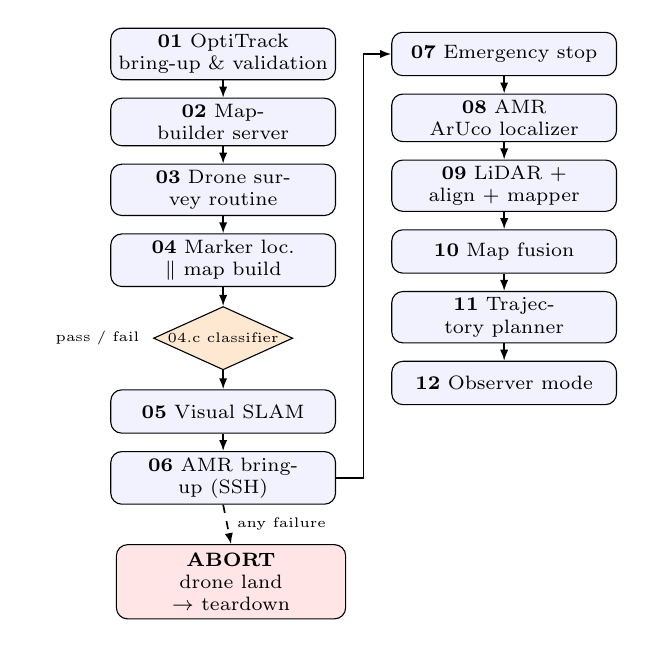
\begin{tikzpicture}[
  font=\scriptsize,
  stage/.style={draw, rounded corners, fill=blue!5, align=center,
                text width=2.7cm, inner sep=2.2pt, minimum height=5.5mm},
  dec/.style={draw, diamond, aspect=2.2, fill=orange!18, align=center,
              inner sep=0pt, text width=1.5cm, font=\tiny},
  term/.style={draw, rounded corners, fill=red!10, align=center,
               text width=2.7cm, inner sep=3pt},
  arr/.style={-{Latex[length=1.4mm]}, semithick}
]
% left column 01..06
\node[stage] (s1) {\textbf{01} OptiTrack bring-up \& validation};
\node[stage, below=2.2mm of s1] (s2) {\textbf{02} Map-builder server};
\node[stage, below=2.2mm of s2] (s3) {\textbf{03} Drone survey routine};
\node[stage, below=2.2mm of s3] (s4) {\textbf{04} Marker loc.\ $\parallel$ map build};
\node[dec, below=2.4mm of s4] (cls) {04.c classifier};
\node[stage, below=2.4mm of cls] (s5) {\textbf{05} Visual SLAM};
\node[stage, below=2.2mm of s5] (s6) {\textbf{06} AMR bring-up (SSH)};
% right column 07..12
\node[stage, right=7mm of s1] (s7) {\textbf{07} Emergency stop};
\node[stage, below=2.2mm of s7] (s8) {\textbf{08} AMR ArUco localizer};
\node[stage, below=2.2mm of s8] (s9) {\textbf{09} LiDAR + align + mapper};
\node[stage, below=2.2mm of s9] (s10) {\textbf{10} Map fusion};
\node[stage, below=2.2mm of s10] (s11) {\textbf{11} Trajectory planner};
\node[stage, below=2.2mm of s11] (s12) {\textbf{12} Observer mode};
% spines
\foreach \a/\b in {s1/s2,s2/s3,s3/s4,s4/cls,cls/s5,s5/s6}\draw[arr](\a)--(\b);
\foreach \a/\b in {s7/s8,s8/s9,s9/s10,s10/s11,s11/s12}\draw[arr](\a)--(\b);
\draw[arr] (s6.east) -- ++(3.5mm,0) |- (s7.west);
\node[font=\tiny, left=0.5mm of cls, text width=1.3cm, align=right]
      {pass / fail};
% abort sink
\node[term, below=5mm of s6, xshift=1mm] (ab)
      {\textbf{ABORT}\\drone land $\to$ teardown};
\draw[arr, dashed] (s6.south) -- (ab.north)
      node[midway, right, font=\tiny] {any failure};
\end{tikzpicture}
\caption{Mission orchestrator state machine. Stages advance left-to-right,
top-to-bottom (01--06 then 07--12). The map-quality classifier (04.c) is the
sole branch: \textsc{pass} routes the planner to \texttt{/drone/map} with a goal
pose; \textsc{fail} publishes a border-template map and arms the
frontier-exploration fallback (11.b, triggered at 12.a). Any sub-stage failure
transitions to the ABORT sink, which lands the drone before tearing down.}
\label{fig:fsm}
\end{figure}

\FIG{Pipeline data-flow with message types at stage boundaries}

%==============================================================================
%  VI. UAV FLIGHT CONTROL
%==============================================================================
\section{UAV Flight Control}
\label{sec:uav-control}

\subsection{Role and Requirements}
\subsys{tello\_pos\_control} flies the survey pattern that
Section~\ref{sec:stitching} stitches into a map, satisfying FR-2. It must track a
world-frame scan trajectory using OptiTrack pose feedback, despite the Tello
exposing only a \emph{body-frame} velocity interface for its control, and must abort safely on
loss of tracking (FR-6) or direct orchestrator's command.

\subsection{Theory and Design Rationale \checked}
\subsubsection{Flight state machine}
Flight proceeds through six states: pre-flight, takeoff/home, stabilize at home,
trajectory, return home, and normal land, with a seventh fault-land state
reachable from the stabilize, trajectory, and return states when the tracking
fault detector fires at detection of unphysical pose data.

\subsubsection{Position controller}
The world-frame position error is $\mathbf{e}=\mathbf{p}-\mathbf{p}^\star$. Each
axis uses PID with feedforward and anti-windup on the integral term,
\begin{equation}
I_{x,k}=\mathrm{clip}\!\left(I_{x,k-1}+e_x\Delta t,\,-I_x^{\max},\,I_x^{\max}\right),
\end{equation}
\begin{equation}
v_x^W=-k_{p,x}e_x-k_{d,x}\tilde{v}_x-k_{i,x}I_x+v_{ff,x},
\end{equation}
where $\tilde{v}_x$ is an EMA-smoothed finite-difference velocity. Because the
Tello accepts body-frame commands, the world-frame command is rotated through
the measured yaw $\psi$:
\begin{equation}
\begin{pmatrix}v_x^B\\v_y^B\end{pmatrix}
=\Rmat(\psi)^\top\begin{pmatrix}v_x^W\\v_y^W\end{pmatrix}
=\begin{pmatrix}\cos\psi&\sin\psi\\-\sin\psi&\cos\psi\end{pmatrix}
\begin{pmatrix}v_x^W\\v_y^W\end{pmatrix}.
\end{equation}
The command is then saturated in a direction-preserving manner at $v_{\max}$, and
yaw is held with $\omega_z=\mathrm{clip}\!\left(-k_{p,\psi}\,\mathrm{atan2}
(\sin(\psi-\psi_d),\cos(\psi-\psi_d)),-1,1\right)$.

\subsubsection{OptiTrack fault detector}
Tracking can fail in an \emph{alternating-ghost} mode, interleaving valid and
corrupted samples, which defeats a naive consecutive-bad-sample counter. We
instead monitor a sliding-window bad-sample ratio. With
$b_k=\mathbf{1}\!\left[\lVert\mathbf{p}_k-\mathbf{p}_{k-1}\rVert>\delta_\text{thr}\right]$,
a fault is declared (and latched) when
\begin{equation}
\hat\rho_k=\frac{1}{W}\sum_{j} b_j > \rho_\text{thr}.
\end{equation}
The detector is active only in the stabilize, trajectory, and return states.

\subsubsection{Scan trajectory}
Survey waypoints form a boustrophedon (lawnmower) raster. The path is
arc-length parameterized, $t_i=s_i/v$ with $s_i=\sum d_j$ the cumulative chord
length, and interpolated by a clamped cubic spline with zero endpoint
velocities. The analytic spline derivative supplies the feedforward velocity.

\subsection{Implementation}
The node subscribes to OptiTrack pose and publishes body-frame velocity commands
to \subsys{tello\_driver}, advancing the state machine on a fixed timer.
\TODO{Topic/parameter table.}

\subsection{Traceability and Tests}
Satisfies FR-2, FR-6, FR-8. \TODO{Flight tests: trajectory tracking error under
nominal tracking; fault-injection test forcing the alternating-ghost mode.}
\FIG{Commanded vs.\ OptiTrack trajectory}

%==============================================================================
%  VII. AERIAL MAPPING AND IMAGE STITCHING
%==============================================================================
\section{Aerial Mapping and Image Stitching}
\label{sec:stitching}

\subsection{Role and Requirements}
\subsys{arena\_map\_builder} converts downward UAV video into a metric occupancy
grid at \SI{5}{\centi\meter}/cell, plus marker positions and a diagnostic feature
vector. It satisfies FR-2 and FR-5 and must fit the Jetson memory budget (NFR-5).

\subsection{Theory and Design Rationale}
\subsubsection{Similarity transform over full homography}
Top-down flight over a planar arena is a 4-DOF rigid-plus-scale motion. A full
8-DOF homography has extra degrees of freedom that RANSAC will use to fit the
repetitive blue-tape grid, producing compounding ``fan'' artifacts across the
hundreds of frames of a survey. We therefore estimate a similarity transform
\begin{equation}
\mathbf{H}_\text{sim}=\begin{pmatrix}a&-b&t_x\\ b&a&t_y\\ 0&0&1\end{pmatrix},
\quad a=s\cos\theta,\; b=s\sin\theta,
\end{equation}
via \texttt{estimateAffinePartial2D} with RANSAC, promoted to $3\times3$ for
composition onto the global canvas.

\subsubsection{Feature extraction with exclusion masking}
The production front-end is SIFT (5000 keypoints/frame, 128-D descriptors). The
arena's blue adhesive grid is masked out by an HSV threshold (dilated
\SI{5}{px}) before detection: without this mask, RANSAC latches onto
visually identical inter-cell tape junctions and converges on the wrong cell. A
GPU alternative front-end uses SuperPoint (256-D) with LightGlue matching,
exported to ONNX and run on the Jetson GPU---the embedded deep-learning component
of the system.

\subsubsection{Matching pipeline}
Frame pairs are matched by (i)~$k$-nearest-neighbour ($k{=}2$) L2 matching,
(ii)~Lowe's ratio test at $r=0.65$, (iii)~a mutual cross-check requiring the
ratio test to pass in both directions, and (iv)~a median-absolute-deviation (MAD)
displacement pre-filter that removes wrong-cell clusters \emph{before} RANSAC:
\begin{equation}
\bm{\mu}=\operatorname*{median}_i(\bm{\Delta}_i),\quad
\mathrm{MAD}=\operatorname*{median}_i\lVert\bm{\Delta}_i-\bm{\mu}\rVert,
\end{equation}
keeping match $i$ iff $\lVert\bm{\Delta}_i-\bm{\mu}\rVert<\kappa\cdot\mathrm{MAD}$
with $\kappa=4.0$. Survivors feed a similarity RANSAC (threshold \SI{3}{px},
5000 iterations, confidence $0.999$).

\subsubsection{Canvas and blending}
A fixed $8000\times8000$ canvas is pre-allocated; each frame is warped only over
its region of interest (${\sim}\SI{6}{\mega\byte}$ vs.\ ${\sim}\SI{140}{\mega\byte}$
for the full canvas). Frames are merged with a 4-level Laplacian pyramid blend
whose weight $\alpha(p)=d_\text{new}/(d_\text{new}+d_\text{old})$ comes from a
dual distance transform, placing the seam along the iso-depth contour.

\subsubsection{Obstacle transfer and consistency scoring}
Obstacles (pink) and walls (green/brown) are transferred by two independent
projections (bounding-box and grid), whose centroid and area agreement form
confidence proxies $s_A,s_B$; a perturbation-stability proxy $s_C$ completes a
weighted score
\begin{equation}
c=\frac{w_A s_A+w_B s_B+w_C s_C}{w_A+w_B+w_C},
\end{equation}
with $(w_A,w_B,w_C)=(0.45,0.25,0.30)$. Occupancy is rasterized with confidence
-weighted halos of width $t(c)=t_\text{base}e^{-3c}$ interpolating from free
to occupied around each obstacle core.

\subsubsection{Learned map-quality gate}
A RandomForest classifier consumes a 45-feature diagnostic vector and outputs a
binary ``map acceptable'' decision $P(\text{pass}\mid\mathbf{f})\geq\tau$.
Inference is pure NumPy (a serialized \texttt{forest.npz}, no scikit-learn at
runtime); missing features map to a $-1$ sentinel for safe-fail. A rejected map
triggers the frontier-exploration fallback of the mission FSM.

\subsection{Implementation}
The builder runs online (incrementally during flight, hiding stitching latency
behind flight time) or offline (post-landing on saved video). Memory is bounded
(NFR-5) by a streaming frame generator, the pre-allocated canvas, ROI warping, a
keyframe cap of 20, and periodic \texttt{malloc\_trim}; peak working set is
${\sim}\SI{287}{\mega\byte}$. A 335-configuration parameter sweep fixed the
deployed baseline (SIFT, $r{=}0.65$, $\kappa{=}4.0$, lookback~8, keyframe
interval~10, processing scale~0.5, blue-tape exclusion).

\subsection{Traceability and Tests}
Satisfies FR-2, FR-5, FR-11, NFR-5. \TODO{Coverage and obstacle TP/FP metrics;
ablations: mask on/off, SIFT vs.\ SuperPoint.}
\FIG{Stitched map with/without exclusion mask}
\FIG{Occupancy grid with confidence halos}

%==============================================================================
%  VIII. AERIAL MARKER LOCALIZATION
%==============================================================================
\section{Aerial Marker Localization}
\label{sec:aruco}

\subsection{Role and Requirements}
\subsys{arena\_marker\_localizer} estimates the world-frame pose of each ArUco
goal marker from the UAV's aerial video and synchronized OptiTrack log,
satisfying FR-3. Position is taken from the stitcher (whose metric pixel
projection is more accurate) and \emph{orientation} from PnP, which depends only
on relative image geometry and is unaffected by map-origin shifts.

\subsection{Theory and Design Rationale}
\subsubsection{Mirror rig and camera transform}
A $45^\circ$ mirror redirects the forward camera to nadir. The calibrated
camera-to-drone transform applies a roll of $\pi$ (mapping the forward optical
axis to downward) and a yaw of \SI{0.0456}{\radian} ($2.6^\circ$ mounting
misalignment), with a small translational lever arm.

\subsubsection{Planar PnP}
Each detected marker yields four corner correspondences solved by IPPE\_SQUARE,
a closed-form planar method that reduces the $3$D--$2$D problem to a homography
and recovers two candidate poses (the planar ambiguity), selecting the one with
lower reprojection error. Detections with reprojection error above
\SI{4}{px} are discarded.

\subsubsection{Transform chain}
A marker pose is composed along a four-link chain,
\begin{equation}
\Tmat_{\text{map}\leftarrow\text{marker}}=
\Tmat_{\text{map}\leftarrow\text{opti}}\,
\Tmat_{\text{opti}\leftarrow\text{drone}}(t)\,
\Tmat_{\text{drone}\leftarrow\text{cam}}\,
\Tmat_{\text{cam}\leftarrow\text{marker}}(t),
\end{equation}
with all links as $4\times4$ homogeneous transforms and the OptiTrack log aligned
row-by-row to video frames.

\subsubsection{Robust aggregation}
Each marker accrues 120--180 observations. These pass a per-axis and circular
MAD gate ($k=3.5$), after which position is aggregated by the Weiszfeld
geometric median (breakdown point ${\sim}50\%$),
$\mathbf{x}^{(k+1)}=\sum_i w_i\mathbf{p}_i/\sum_i w_i$ with $w_i=1/\lVert
\mathbf{p}_i-\mathbf{x}^{(k)}\rVert$, and yaw by the circular median
$\hat\theta=\mathrm{atan2}(\operatorname{median}\sin\theta_i,
\operatorname{median}\cos\theta_i)$.

\subsubsection{Bias calibration}
A four-term linear error model---map-origin shift, camera lever arm, radial scale
bias, and yaw misalignment---is fit by iteratively reweighted least squares with
Huber weights and physical bounds, validated by leave-one-scan-out
cross-validation. An SVD condition-number check detects attitude degeneracy and
falls back to a reduced model.

\subsection{Implementation}
The subsystem exposes a \texttt{/localize\_markers} service invoked in mission
Stage~04 as the orientation source, joined with the map-builder position to
publish \texttt{/aruco/amr/pose} and (on classifier pass)
\texttt{/aruco/goal/pose}. \TODO{Service/message interface details.}

\subsection{Traceability and Tests}
Satisfies FR-3, FR-9. \TODO{Position and yaw error after calibration;
cross-validation residuals.}
\FIG{Transform-chain and mirror-rig geometry diagram}

%==============================================================================
%  IX. AMR STATE ESTIMATION (EKF)
%==============================================================================
\section{AMR State Estimation: Extended Kalman Filter}
\label{sec:ekf}

\subsection{Role and Requirements}
\subsys{ekf\_amr} is the AMR's state estimator, fusing wheel-encoder velocity,
IMU gyroscope, and visual-odometry (VIO) forward velocity into a continuous pose
on \texttt{/amr/ekf/odom} and the $\texttt{odom}\to\texttt{base\_footprint}$
transform. It is implemented from scratch (NFR-1). The GPS-denied design (no
absolute-positioning markers on the AMR) forces the estimate to be built from
proprioceptive and onboard sensing alone; the noisy, loop-closure-spiked VIO
stream demands adaptive gating that stock packages do not provide.

\subsection{Theory and Design Rationale}
\subsubsection{State and process model}
The state $\state=[x,y,\theta,v,\omega]^\top$ carries velocity as explicit states
so heterogeneous velocity sources---and future absolute-position fixes---all
enter through standard Kalman updates. Between steps it evolves under a unicycle
model with a constant-velocity assumption,
\begin{equation}
f(\state)=\big[\,x+T_s v\cos\theta,\;y+T_s v\sin\theta,\;\theta+T_s\omega,\;v,\;\omega\,\big]^\top,
\end{equation}
with Jacobian
\begin{equation}
F=\begin{pmatrix}
1&0&-T_s v\sin\theta&T_s\cos\theta&0\\
0&1& T_s v\cos\theta&T_s\sin\theta&0\\
0&0&1&0&T_s\\
0&0&0&1&0\\
0&0&0&0&1
\end{pmatrix},
\end{equation}
and process noise $Q=\mathrm{diag}(10^{-4},10^{-4},10^{-4},0.05,0.05)$: pose is
trusted to propagate, while loose velocity noise lets measurements correct
$(v,\omega)$ freely. The prediction is $\hat\state^-=f(\state_{k-1})$,
$P^-=FPF^\top+Q$, with heading wrapped to $(-\pi,\pi]$.

\subsubsection{Measurement updates}
Three updates fire sequentially each step (wheel, IMU, VIO), skipping sensors
with no new reading. Wheel odometry observes $(v,\omega)$ with
$R_\text{wheel}=\mathrm{diag}(0.2,0.2)$ (slip and quantization). The IMU observes
$\omega$ after subtracting a calibrated bias $b=\SI{0.002618}{\radian\per\second}$,
with a tight $R_\text{imu}=\mathrm{diag}(0.001)$. VIO contributes only its
forward velocity $v_{x,\text{vio}}$ ($R_\text{vio}=\mathrm{diag}(0.1)$); its
position is discarded because VSLAM position drifts and jumps at loop closures.

\subsubsection{Adaptive VIO gate}
A fixed-cutoff Butterworth low-pass filter could not suppress loop-closure
spikes---its transient response to a sharp spike propagated into the filter and
caused sustained position deviations. The deployed \texttt{ema\_gate} is a
two-stage adaptive filter. Stage~P0 holds the last good value when
$|v_x|>\SI{0.5}{\meter\per\second}$ (the robot's mechanical limit). Stage~P1
tracks online EMA estimates of mean and variance,
\begin{equation}
\hat\mu_k=\alpha v_k+(1-\alpha)\hat\mu_{k-1},\quad
\widehat{v^2}_k=\alpha v_k^2+(1-\alpha)\widehat{v^2}_{k-1},
\end{equation}
$\hat\sigma^2=\max(0,\widehat{v^2}-\hat\mu^2)$, and gates against
$\tau_k=\max(2.0\,\hat\sigma_k,\,0.17)$, the floor preventing collapse near
standstill. Because spikes arrive in clusters, a 10-sample window of spike
decisions triggers \emph{burst mode} above a $0.30$ spike fraction, during which
all samples are rejected and the statistics update slowly
($\alpha_\text{burst}=0.02$). A 20-sample warmup seeds the statistics.

\begin{algorithm}[t]
\caption{P1 adaptive EMA gate (per VIO sample)}
\label{alg:emagate}
\begin{algorithmic}
\STATE $\textit{in\_burst}\leftarrow \mathrm{mean}(\textit{recent\_window})\geq 0.30$
\STATE $\sigma^2\leftarrow\max(0,\,\textit{ema\_sq}-\textit{ema}^2)$
\STATE $\tau\leftarrow\max(2.0\sqrt{\sigma^2},\,0.17)$
\STATE $\textit{spike}\leftarrow |v_x-\textit{ema}|>\tau$
\IF{$\textit{in\_burst}$ \OR $\textit{spike}$}
  \STATE $v_\text{out}\leftarrow\textit{last\_good}$
  \STATE update $\textit{ema},\textit{ema\_sq}$ with $\alpha_\text{burst}$, $\mathrm{clip}(v_x,-0.5,0.5)$
\ELSE
  \STATE $\textit{last\_good}\leftarrow v_x$;\quad $v_\text{out}\leftarrow v_x$
  \STATE update $\textit{ema},\textit{ema\_sq}$ with $\alpha$, $v_x$
\ENDIF
\STATE append $\textit{spike}$ to $\textit{recent\_window}$;\quad \textbf{return} $v_\text{out}$
\end{algorithmic}
\end{algorithm}

\subsubsection{Covariance update and anchoring}
All updates use the Joseph form
$P^+=(I-KH)P^-(I-KH)^\top+KRK^\top$, preserving symmetry and positive
semi-definiteness to machine precision. No active sensor observes absolute
$(x,y)$, so the filter dead-reckons between fixes; the 5-state form admits an
ArUco position update $H_\text{aruco}=[I_{3\times3}\,|\,0_{3\times2}]$ with no
structural change.

\subsection{Implementation}
The EKF step runs on a fixed \SI{100}{\hertz} timer independent of sensor arrival;
callbacks buffer readings behind \texttt{\_new} flags, and a step with no new
data returns early to avoid spurious drift. Parameters appear in
Table~\ref{tab:ekf}.

\begin{table}[t]
\caption{EKF Deployed Parameters (selected)}
\label{tab:ekf}
\centering
\begin{tabular}{@{}lll@{}}
\toprule
\textbf{Parameter} & \textbf{Value} & \textbf{Meaning} \\
\midrule
\texttt{sampling\_time} & \SI{0.01}{\second} & step period (\SI{100}{\hertz}) \\
$Q$ diag & $[10^{-4}{,}10^{-4}{,}10^{-4}{,}0.05{,}0.05]$ & process noise \\
$R_\text{wheel}$ & $[0.2,0.2]$ & wheel $[v,\omega]$ \\
$R_\text{imu}$ & $[0.001]$ & gyro $[\omega]$ \\
$R_\text{vio}$ & $[0.1]$ & VIO $[v_x]$ \\
\texttt{p0\_vx\_max} & \SI{0.5}{\meter\per\second} & physical limit \\
\texttt{p1\_n\_sigma} & $2.0$ & gate width \\
\texttt{p1\_burst\_thresh} & $0.30$ & burst entry fraction \\
\bottomrule
\end{tabular}
\end{table}

\subsection{Traceability and Tests}
Satisfies FR-1, FR-10, NFR-1, NFR-7. \TODO{Position RMSE vs.\ OptiTrack ground truth; VIO
spike-rejection ablation (gate on/off).}
\FIG{EKF state and covariance traces over a run}
\FIG{Raw vs.\ gated VIO velocity}

%==============================================================================
%  X. AMR DRIVE STACK
%==============================================================================
\section{AMR Drive Stack: Odometry and Control}
\label{sec:drive}

\subsection{Role and Requirements}
\subsys{amr\_bringup} is the RDK~X3 hardware layer: \subsys{driver\_node}
(hardware abstraction), \subsys{wheel\_odometry\_node} (dead-reckoning), and
\subsys{controller\_node} (reference tracking). Together they close a
sensing--estimation--control loop at the drive level, decoupled from planning.

\subsection{Theory and Design Rationale}
\subsubsection{Hardware abstraction}
\subsys{driver\_node} wraps the SunriseRobot SDK and is the only node touching
hardware. It forwards \texttt{/amr/cmd\_vel} to \texttt{set\_car\_motion}, reads
wheel velocity, IMU, and battery at \SI{100}{\hertz}, and enforces emergency
stop: a \texttt{False}$\to$\texttt{True} transition immediately commands zero
motion and a three-beep alert; the clear transition resumes commands. The IMU is
mounted non-canonically, so a fixed axis permutation and sign flip maps the SDK
frame to the ROS body frame,
\begin{equation}
(a_x,a_y,a_z)_\text{ROS}=(-a_x^s,\,a_z^s,\,a_y^s),
\end{equation}
and identically for the gyroscope; the magnetometer is unused.

\subsubsection{Dead-reckoning odometry}
Though mechanically a mecanum platform, the base is treated as a differential
-drive robot: lateral velocity is discarded ($\dot{y}_\text{body}=0$ by
construction), since planning never commands lateral motion. The pose integrates
by Euler,
\begin{equation}
x_{k+1}=x_k+v_x\cos\theta_k\Delta t,\;\;
y_{k+1}=y_k+v_x\sin\theta_k\Delta t,
\end{equation}
$\theta_{k+1}=\mathrm{wrap}(\theta_k+\omega_z\Delta t)$, with a $\Delta t$ guard
($0<\Delta t\leq\SI{1}{\second}$) and unit calibration scales (the SDK velocities
need no correction at the arena scale).

\subsubsection{Feedback-linearizing controller}
The planner publishes a world-frame reference $(x_r,y_r,\theta_r)$ with velocity
$(\dot{x}_r,\dot{y}_r)$. Controlling the centre directly is singular for the
unicycle, so the controller acts on a virtual point $R=\SI{0.2}{\meter}$ ahead,
$x_R=x+R\cos\theta$, $y_R=y+R\sin\theta$. Virtual proportional-plus-feedforward
inputs $u_1=k_{px}(x_r-x_R)+\dot{x}_r$, $u_2=k_{py}(y_r-y_R)+\dot{y}_r$
($k_{px}=1.0$, $k_{py}=2.0$) are mapped to body commands by inverting
\begin{equation}
\begin{pmatrix}\dot{x}_R\\\dot{y}_R\end{pmatrix}=
\underbrace{\begin{pmatrix}\cos\theta&-R\sin\theta\\\sin\theta&R\cos\theta\end{pmatrix}}_{T(\theta)}
\begin{pmatrix}v\\\omega\end{pmatrix},
\end{equation}
which is invertible everywhere ($\det T=R\neq0$), giving
$v=u_1\cos\theta+u_2\sin\theta$ and $\omega=(-u_1\sin\theta+u_2\cos\theta)/R$ and
the decoupled error dynamics $\dot{e}_x=-k_{px}e_x$, $\dot{e}_y=-k_{py}e_y$.
Drivetrain stiction is compensated by a deadband offset,
$v_\text{cmd}=\mathrm{sgn}(v)(|v|+0.15)$ for $|v|>\SI{0.001}{\meter\per\second}$.

\subsection{Implementation}
The controller reads pose from the $\texttt{world}\to\texttt{base\_footprint}$
transform rather than a fixed odometry topic, making it localization-agnostic;
all three nodes run \SI{100}{\hertz} loops.

\subsection{Traceability and Tests}
Satisfies FR-1, FR-4 (emergency-stop actuation), NFR-7. \TODO{Step-response and
tracking-error tests.}

%==============================================================================
%  XI. LIDAR SENSING AND OCCUPANCY MAPPING
%==============================================================================
\section{LiDAR Sensing and Occupancy Mapping}
\label{sec:mapping}

\subsection{Role and Requirements}
\subsys{oradar\_ros} drives the LiDAR and \subsys{world\_mapper} maintains the
AMR's running occupancy map, jointly satisfying FR-4 and NFR-2.

\subsection{Theory and Design Rationale}
\subsubsection{LiDAR driver}
The OraDAR MS200 streams \texttt{OradarLidarFrame} packets (12 points each,
CRC-8 checked, distances in mm, angles in centi-degrees). The driver converts
clockwise to counter-clockwise ($\textit{angle}\to360-\textit{angle}$), gates
ranges to \SIrange{0.05}{20}{\meter}, maps returns onto a regular angular grid
(nearest return wins on collision), and fills single-cell gaps by interpolation.
A static transform places the sensor at $x=\SI{0.07}{\meter}$,
$z=\SI{0.13}{\meter}$ on \texttt{base\_footprint}; the scan timestamp is the
acquisition start, bounding positional uncertainty to ${\leq}\SI{10}{\milli\meter}$
at operating speed.

\subsubsection{Bayesian occupancy update}
Each cell holds a log-odds value updated additively,
$l_t=l_{t-1}+l_\text{sensor}-l_0$ with $l_0=0$, using $l_\text{occ}=+0.85$ and
$l_\text{free}=-0.40$. The $2.1{:}1$ asymmetry encodes that an occupied return is
more informative than a free one. Beams are integrated by Bresenham ray casting:
cells along the beam receive the free increment and the terminal cell (if in
range) the occupied increment. Values saturate, so cells require several
consistent observations to commit (${\sim}6$ hits or $13$ misses).

\subsubsection{Handling of dynamic obstacles}
The arena contains only static obstacles, so no motion model or prediction is
implemented. A slowly moving obstacle is nonetheless handled---sub-optimally but
without any dedicated machinery---by the continuous log-odds update itself: as the
obstacle vacates a cell, repeated free returns drive that cell's log-odds back
below the occupancy threshold, while its new location accumulates occupied
returns. The hit/miss asymmetry and saturation bounds set how quickly the map
forgets a departed obstacle; this lag makes the scheme adequate only for motion
slow relative to the mapping rate (FR-13).

\subsection{Implementation}
The driver runs at the deployed \SI{15}{\hertz}; \subsys{world\_mapper} integrates
scans on a \SI{50}{\hertz} timer along the
$\texttt{world}\to\texttt{odom}\to\texttt{base\_footprint}\to\texttt{lidar}$
chain. The $\texttt{world}\to\texttt{odom}$ transform is published by the
\subsys{alignment\_node} from the drone-observed AMR fix on
\texttt{/aruco/amr/pose} (Stage~09.b); when that pose is unavailable it arrives
as all-NaN, which the alignment node reads as ``no data'' and replaces with the
trivial identity transform.

\subsection{Traceability and Tests}
Satisfies FR-4, FR-9, FR-13, NFR-2. \TODO{Mapping fidelity vs.\ ground-truth
obstacle layout.}
\FIG{Live occupancy map during a run}

%==============================================================================
%  XII. MAP FUSION
%==============================================================================
\section{Map Fusion}
\label{sec:fusion}

\subsection{Role and Requirements}
\subsys{fusion} merges the aerial prior with the AMR's live LiDAR map into the
costmap the planner consumes (FR-4, FR-5).

\subsection{Theory and Design Rationale}
Both maps are published in the same \texttt{world} frame at identical resolution
and origin by construction, so \emph{no registration is needed}. Fusion is a
single vectorized elementwise pass with a four-case priority rule (drone
threshold $65$, default fill $25$):
\begin{equation}
G_F=\begin{cases}
100 & G_D\geq 65\ \text{(drone obstacle, immutable)}\\
G_A & G_D=-1\ \text{(drone unknown, defer to AMR)}\\
\max(25,G_A) & G_D<65,\,G_D\neq-1,\,G_A\neq-1\\
25 & \text{otherwise.}
\end{cases}
\end{equation}
Drone free space is treated as $25$ rather than $0$ because aerial stitching is
not certain enough to assert free; the AMR map can only \emph{raise} occupancy,
never clear a drone obstacle. An earlier ICP-based registration was abandoned:
early in a mission the AMR map is too sparse for stable coarse-search peaks, and
exact pre-alignment made registration unnecessary.

\subsection{Implementation}
The drone map uses \texttt{TRANSIENT\_LOCAL} QoS so the node receives it even if
it starts late; the fused map is republished reactively on each AMR update.

\subsection{Traceability and Tests}
Satisfies FR-4, FR-5, NFR-9. \TODO{Fused-map correctness vs.\ individual sources.}
\FIG{Drone / AMR / fused maps side by side}

%==============================================================================
%  XIII. PATH PLANNING AND TRAJECTORY EXECUTION
%==============================================================================
\section{Path Planning and Trajectory Execution}
\label{sec:planner}

\subsection{Role and Requirements}
\subsys{trajectory\_planner} plans a collision-free path to the goal and emits a
trackable reference for the drive stack (FR-1, FR-4, NFR-3).

\subsection{Theory and Design Rationale}
The fused costmap is inflated by an exponential look-up table
$c(d)=99\,e^{-k(d-r_\text{robot})}$ ($k=3.5$, saturating to 100 inside the robot
radius). A$^\star$ searches the 8-connected grid with the octile heuristic
\begin{equation}
h=\max(\Delta x,\Delta y)+(\sqrt2-1)\min(\Delta x,\Delta y),
\end{equation}
on occupancy-weighted edge costs. Replanning triggers on goal change, path
blockage, elapsed time, or a proximity score $\sigma_\text{prox}=\sum_i
e^{-d_i/r}$ exceeding a threshold. The waypoint path is smoothed by an arc-length
-parameterized cubic spline and given a trapezoidal speed profile (ramp distance
$d_\text{ramp}=v^2/2a=\SI{0.225}{\meter}$)---the dynamic speed adjustment of the
extra-credit criteria. The resulting reference is tracked by the same
feedback-linearizing controller as Section~\ref{sec:drive}.

\subsection{Implementation}
Inputs are the fused \texttt{/drone/map} and the ArUco goal pose; the node
publishes the time-parameterized reference to the drive controller.

\subsection{Traceability and Tests}
Satisfies FR-1, FR-4, FR-13, NFR-3. \TODO{Path optimality, replanning latency,
dynamic-obstacle response.}
\FIG{Planned path over inflated costmap}

%==============================================================================
%  XIV. AUTOMATIC EMERGENCY BRAKING
%==============================================================================
\section{Physical Safety: Automatic Emergency Braking}
\label{sec:aeb}

\subsection{Role and Requirements}
\subsys{emergency\_stop} is an independent, high-rate safety layer decoupled from
planning (FR-4, NFR-4).

\subsection{Theory and Design Rationale}
A blind-spot angular mask excludes $[120^\circ,240^\circ]$ (chassis structure).
An $N$-consecutive streak detector commands STOP after $n=5$ consecutive scans
report an obstacle within \SI{0.3}{\meter}, and clears after $n$ clean scans;
at the deployed \SI{15}{\hertz} this is a reaction time of
$\tau\approx5/15\approx\SI{333}{\milli\second}$. Multiple trigger reasons combine
in an OR state machine. Safety holds when the stopping distance bound
$d_{\min}>v\cdot(n/f_s)+d_\text{brake}$ is satisfied.

\subsection{Implementation}
The node raises \texttt{/amr/emergency\_stop}, which \subsys{driver\_node} honors
by zeroing motion; the mission FSM health-checks the node at Stage~07.

\subsection{Traceability and Tests}
Satisfies FR-4, FR-12, NFR-4. \TODO{Measured response time; false-trigger rate.}

%==============================================================================
%  XV. NETWORK SECURITY MIDDLEWARE
%==============================================================================
\section{Network Security Middleware}
\label{sec:security}

\subsection{Role and Requirements}
\subsys{ros2\_security} authenticates and optionally encrypts ROS~2 traffic
without DDS-Security or SROS2, satisfying FR-7. It is opt-in per node, with a
global kill switch and mixed-trust support.

\subsection{Theory and Design Rationale}
A self-signed CA (RSA-4096) issues per-node RSA-2048 X.509 certificates whose
common name equals the node name; all nodes load the CA certificate to verify
peers. Three levels are offered: \texttt{NONE} (pass-through), \texttt{SIGN}
(RSA-PSS over the CDR payload), and \texttt{SIGN\_ENCRYPT} (AES-256-GCM then
RSA-PSS over the ciphertext). At publish, the payload is serialized, optionally
encrypted with a random 12-byte nonce, signed, and wrapped in a
\texttt{SecureEnvelope} (sender id, timestamp, signature, payload, nonce). At
subscribe, the signature is verified \emph{before} any decryption (no decrypt
oracle), the sender is checked against the trusted set, the \texttt{min\_level}
policy is enforced, the timestamp is checked against a replay window, and only
then is the payload decrypted and deserialized. The AES key is derived
deterministically as $\mathrm{SHA\text{-}256}(\text{public-key DER})$---the only
key material both parties share---so no secret distribution is required. A
\texttt{LegacyRelayNode} bridges secured and native topologies, and the
\texttt{ROS2\_SECURITY\_DISABLED} kill switch degrades the whole system to native
ROS~2 uniformly (a mixed state would cause a DDS type mismatch).

\subsection{Implementation}
Security is added by a \texttt{SecureNodeMixin} drop-in; policy resolves by
priority (kill switch $>$ explicit code argument $>$ YAML policy $>$ global
default). Certificates are minted once per deployment.

\subsection{Traceability and Tests}
Satisfies FR-7, NFR-10, NFR-11. \TODO{Unit and integration suite results: tamper, replay, and
wrong-sender rejection; SIGN\_ENCRYPT round-trip; per-message overhead.}

%==============================================================================
%  XVI. EXPERIMENTAL RESULTS
%==============================================================================
\section{Experimental Results}
\label{sec:results}

\subsection{Experimental Setup}
\TODO{Arena, obstacle configurations, marker placement, ground-truth source
(OptiTrack), number of runs.}

\subsection{Aerial Mapping Accuracy}
\TODO{Coverage, obstacle TP/FP, marker localization error after calibration.}

\subsection{State Estimation Accuracy}
\TODO{EKF position RMSE vs.\ OptiTrack; VIO-gate effectiveness.}

\subsection{Navigation Performance}
\TODO{Goal-reach success rate, path-tracking error, collision count, mission
wall-clock time.}

\subsection{Safety and Security Validation}
\TODO{AEB response time; security test-suite results and overhead.}

\subsection{Discussion}
\TODO{Quantitative improvement metrics; robustness observations; limitations
(dead-reckoning drift between fixes, static gyro bias, sequential-update
approximation).}

%==============================================================================
%  XVII. CONCLUSION
%==============================================================================
\section{Conclusion and Future Work}
\label{sec:conclusion}
We presented a cooperative UAV--AMR system that navigates to a goal in a
GPS-denied, initially unmapped arena by having an aerially positioned drone build
the map and localize the goal, then handing that prior to a ground robot that
fuses it with onboard sensing. The design satisfies the project's functional and
non-functional requirements through a from-scratch EKF, a similarity-transform
stitching pipeline with embedded deep learning, robust marker localization,
registration-free map fusion, an independent emergency-braking layer, and an
application-layer security middleware, all integrated in ROS~2 across three
networked platforms. \TODO{Restate headline results.} Future work includes more
frequent ArUco re-anchoring to bound dead-reckoning drift, online gyro-bias
estimation, dynamic-obstacle prediction in the planner, and scaling to larger
multi-robot teams.

%==============================================================================
%  ACKNOWLEDGMENT
%==============================================================================
\section*{Acknowledgment}
\TODO{Advisors; OMRON Automation; Nuclea Solutions; Tecnológico de Monterrey.}

%==============================================================================
%  REFERENCES
%==============================================================================
\begin{thebibliography}{00}
\bibitem{ros2} \TODO{ROS~2 / DDS reference.}
\bibitem{ekf} \TODO{Thrun, Burgard, Fox --- Probabilistic Robotics (EKF, occupancy grids).}
\bibitem{sift} \TODO{Lowe --- Distinctive image features (SIFT).}
\bibitem{ransac} \TODO{Fischler \& Bolles --- RANSAC.}
\bibitem{ippe} \TODO{Collins \& Bartoli --- IPPE planar pose.}
\bibitem{superpoint} \TODO{DeTone et al.\ --- SuperPoint.}
\bibitem{lightglue} \TODO{Lindenberger et al.\ --- LightGlue.}
\bibitem{astar} \TODO{Hart, Nilsson, Raphael --- A*.}
\bibitem{weiszfeld} \TODO{Weiszfeld --- geometric median.}
\bibitem{repo} \TODO{Project repositories (jetson / rasp / security\_middleware).}
\end{thebibliography}

\end{document}
